\section{РЕЗУЛЬТАТЫ ЖАНРОВОЙ КЛАССИФИКАЦИИ}
\label{sec:genre_classification}



\begin{figure}[h]
\centering
  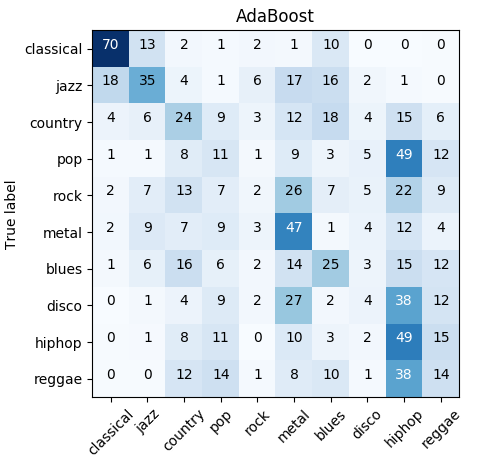
\includegraphics{AdaBoost.png}
  \caption{Матрица ошибок полученная с помощь метода классификации AdaBoost SAMME, где используется <<комитет>>  деревьев принятия решений.}
  \label{fig:results:adaboost}
\end{figure}


\begin{figure}[h]
\centering
  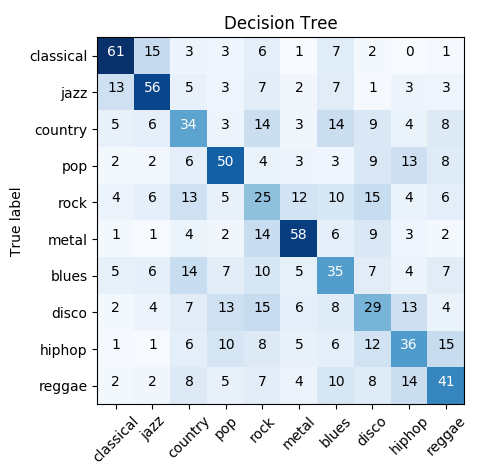
\includegraphics{DecisionTree.png}
  \caption{Матрица ошибок полученная с помощь дерева принятия решения}
  \label{fig:results:DecisionTree}
\end{figure}


\begin{figure}[h]
\centering
  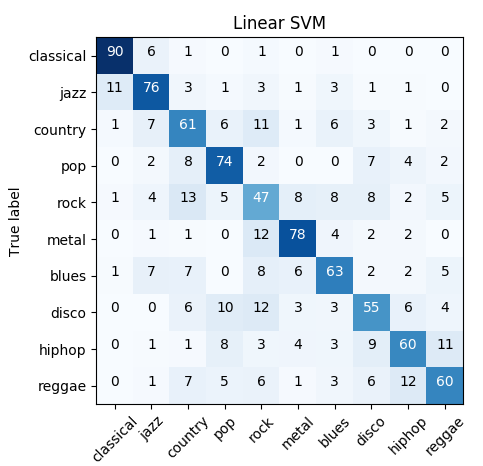
\includegraphics{LinearSVM.png}
  \caption{Матрица ошибок полученная с помощь метода опорных векторов}
  \label{fig:results:LinearSVM}
\end{figure}


\begin{figure}[h]
\centering
  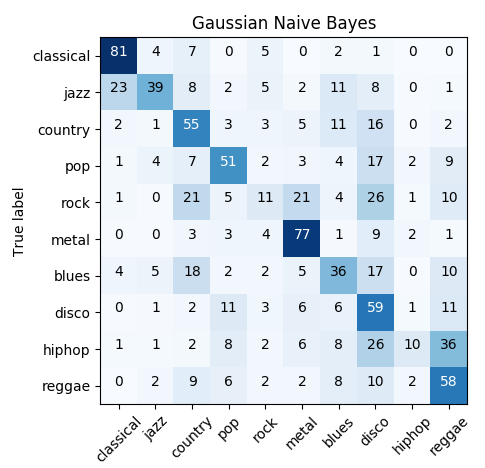
\includegraphics{NaiveBayes.png}
  \caption{Матрица ошибок полученная с помощь наивного баесовского классификатора}
  \label{fig:results:NaiveBayes}
\end{figure}

\begin{figure}[h]
\centering
  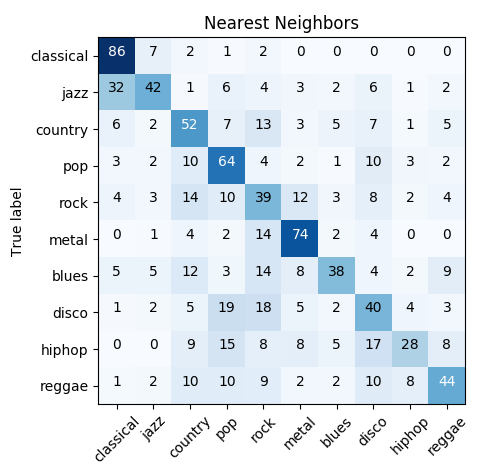
\includegraphics{NearestNeighbors.png}
  \caption{Матрица ошибок полученная с помощь метода k ближайших соседей}
  \label{fig:results:NearestNeighbors}
\end{figure}

\begin{figure}[h]
\centering
  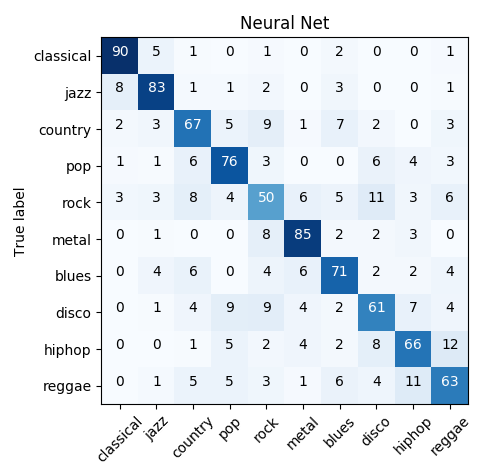
\includegraphics{NeuralNet.png}
  \caption{Матрица ошибок полученная с помощь многослойного перцептрона}
  \label{fig:results:NeuralNet}
\end{figure}


\begin{figure}[h]
\centering
  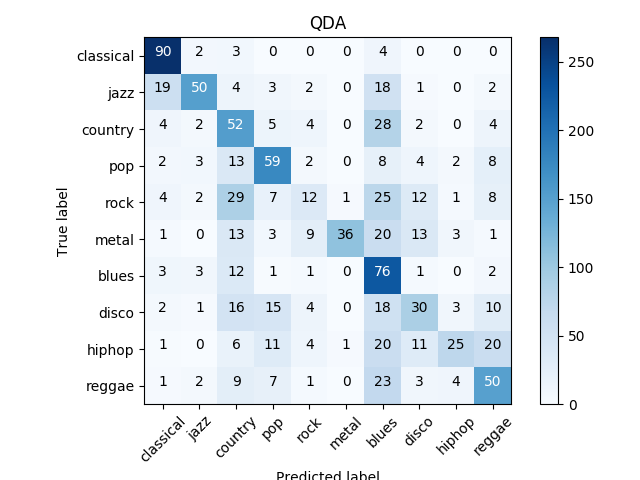
\includegraphics{QDA.png}
  \caption{Матрица ошибок полученная с помощь QDA}
  \label{fig:results:QDA}
\end{figure}


\begin{figure}[h]
\centering
  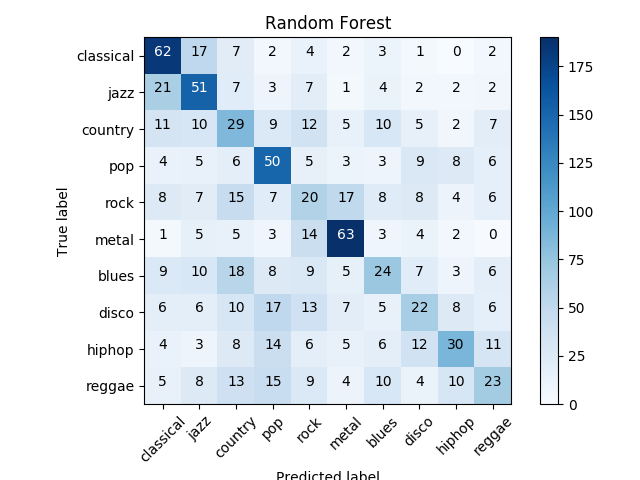
\includegraphics{RandomForest.png}
  \caption{Матрица ошибок полученная с случайного леса}
  \label{fig:results:RandomForest}
\end{figure}








